\chapter{Introduction}

\large{\paragraph{}Stereoscopy (also called stereoscopics, or stereo imaging) is a technique for creating or enhancing the illusion of depth in an image by means of stereopsis for binocular vision[2]. The word stereoscopy derives from Greek στερεός (stereos), meaning 'firm, solid', and σκοπέω (skopeō), meaning 'to look, to see'.}
\large{\paragraph{}Any stereoscopic image is called a stereogram. Originally, stereogram referred to a pair of stereo images which could be viewed using a stereoscope.}
\large{\paragraph{}Most stereoscopic methods present two offset images separately to the left and right eye of the viewer. These two-dimensional images are then combined in the brain to give the perception of 3D depth. This technique is distinguished from 3D displays that display an image in three full dimensions, allowing the observer to increase information about the 3-dimensional objects being displayed by head and eye movements.}\\\\

\begin{figure}[H]
  \centering
    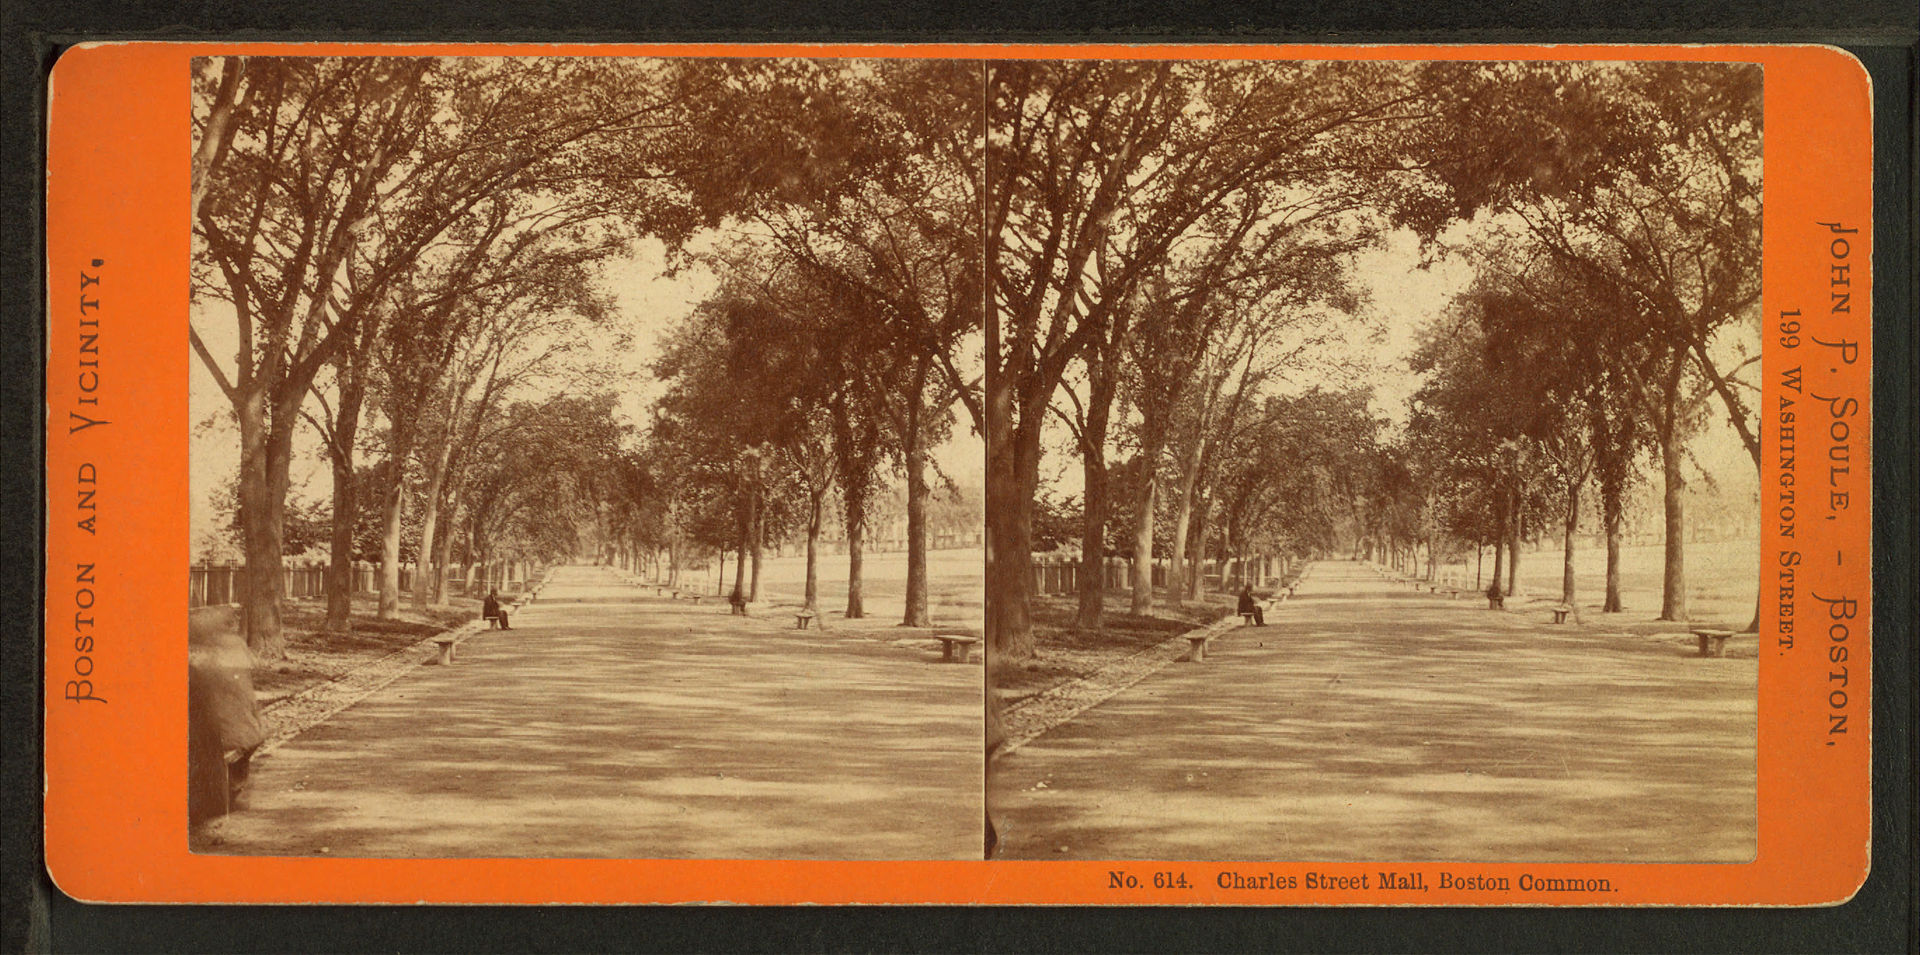
\includegraphics[height= 6cm, width=9cm]{project/images/stereo}
  \caption{\textsc{Stereoscopic Image}}
\end{figure}

